\documentclass[12pt]{scrartcl}
\usepackage{config}
\usepackage{minted}

%\newcommand\mrh{\color{white}\bfseries}
\newcommand\mrc[1]{\begin{tabular}{@{}l@{}} #1 \end{tabular}}
\setlength\arrayrulewidth{0.8pt}

\usemintedstyle{pastie}

\begin{document}
    \hh{Xor Tree}
    
    
    \vspace{10pt}

    
    \hh{Problem}
    
        You are given an integer $N$ and $N - 1$ edges with weights. These edges connect $N$ vertices in such a way that there exists a path\footnote{A path in a graph is defined as a sequence of $k$ vertices $\{v_1, v_2, \cdots , v_k\}$, such that for all $1 \le i \le k - 1$, the edge $\{v_i, v_{i + 1}\}$ exists in the graph. } between any two vertices (i.e. they form a tree).
        
        For each path, we define its weight as the {\bfseries xor} \footnote{Exclusive or, here we define it as the bitwise operation.} of each of the weights of the edges that make up the path. Determine the sum of the weights of all simple paths (paths that do not repeat edges) in the tree \footnote{The path $\{a, b\}$ is considered the same as $\{b, a\}$.}.
        
    \hh{Implementation Details}

        You must implement the function \textit{Encuentra\_xor()}. This function receives an integer $N$, 3 vectors $u, v$, and $w$, each with $N - 1$ elements. For each $0 \le i \le N - 2$, $u[i]$ and $v[i]$ are the vertices connected by edge $i$, and $w[i]$ is its weight. This function must return an integer, the sum of the weights of all the paths.
        The function would look like this:

\begin{minted}{c++}
#include <bits/stdc++.h>
using namespace std;

long long Encuentra_xor(int N, vector<int> u, vector<int> v, vector<int> w) {
    // Implement this function.
}
    
\end{minted}

    The grader will call the function \textbf{multiple} times for each case.

    \hh{Examples}

               
        {\itshape Example 1:}
        
        \begin{itemize}
            \item  The grader calls the function 
            \begin{center}
                \textit{Encuentra\_xor(5, \{0, 1, 0, 4\}, \{1, 2, 3, 1\}, \{2, 3, 4, 0\})}
            \end{center}
            the tree in this case is illustrated in the following image:
            
            \begin{center}
                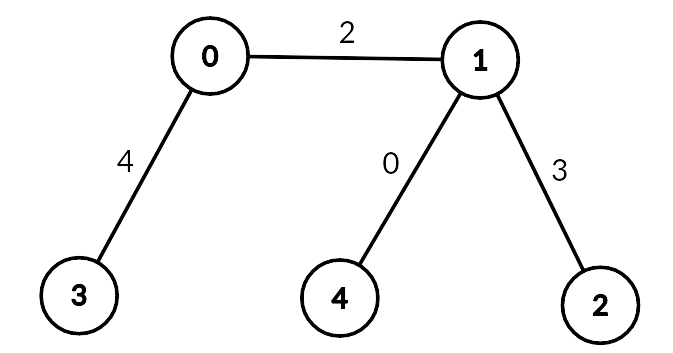
\includegraphics[scale=0.3]{ej1.png}
            \end{center}
            
            \item The xors of the paths are:

                \begin{center}
                    
                \begin{tabular}{|c||c|c|c|c|c|}
                     \hline
                      $\oplus$ & 0 & 1 & 2 & 3 & 4  \\
                     \hline
                     \hline 
                     0 & 0 & 2 & 1 & 4 & 2 \\
                     \hline 
                     1 & 2 & 0 & 3 & 6 & 0 \\ 
                     \hline
                     2 & 1 & 3 & 0 & 5 & 3 \\
                     \hline
                     3 & 4 & 6 & 5 & 0 & 6 \\
                     \hline
                     4 & 2 & 0 & 3 & 6 & 0 \\
                     \hline
                \end{tabular}
                
                \end{center}
            \item  The function must return 32, the sum of the xor of all the paths (the path $\{a, b\}$ is considered the same as $\{b, a\}$).
                
        \end{itemize}


        {\itshape Example 2:}
        \begin{itemize}
            \item The evaluator calls the function 
            \begin{center}
                \textit{Encuentra\_xor(9, \{0, 1, 0, 1, 0, 2, 3, 3\}, \{1, 2, 3, 4, 5, 6, 7, 8\}, \{2, 3, 4, 5, 1, 0, 7, 2\})} 
            \end{center}
            the tree in this case is as follows:

            \begin{center}
                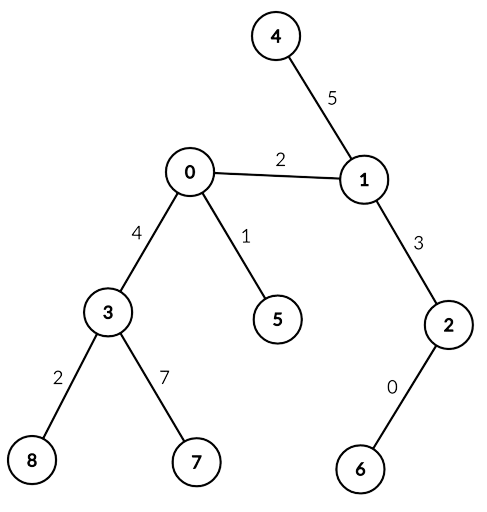
\includegraphics[scale=0.5]{ej2.png}
            \end{center}
            \item The function must return 132.
            
        \end{itemize}
               
        


    
    \hh{Constrains}
        \begin{itemize}
            \item $1 \le N \le 2\times10^5$.
            \item The vectors $u, v$, and $w$ will each have exactly $N - 1$ elements.
            \item For each $0 \le i \le N - 2$, it holds that $0 \le u[i] \neq v[i] < N$. 
            \item For each $0 \le i \le N - 2$, it holds that $0 \le w[i] \le 10^9$.
            \item It is guaranteed that the graph formed by the edges is a tree.
            \item Let $S_N$ be the total sum of the values of $N$ over all the times the function is called during a case. It is guaranteed that $S_N \le 2 \times 10^5$.
        \end{itemize}
    
    \hh{Subtasks}


    \begin{itemize}
        \item (10 points) $N, S_N \le 2000$.
        \item (20 points) For all $0 \le i \le N - 2$, it holds that $w[i] \le 1$.
        \item (25 points) For all $0 \le i \le N - 2$, it holds that $u[i] = i, v[i] = i + 1$.
        \item (45 points) No additional constraints.
    \end{itemize}
\end{document}
